% Fig (methods, estimation) - leakage-free ensemble-Kalman predict-correct loop.
%
% The deployment claim of the paper: the pooled coefficient state is advanced by
% the matched forecast model (predict) and corrected from a sparse set of wall
% pressure taps through the observation operator (correct). No field ever enters
% the loop; the state is the same 32-vector throughout.
%
% Standalone-compilable: pdflatex fig_estimation_loop.tex

\documentclass[border=10pt,tikz]{standalone}
\usepackage{tikz}
\usepackage{amsmath,amssymb}
\usetikzlibrary{positioning,arrows.meta,fit,shapes.geometric,calc,backgrounds}

\begin{document}

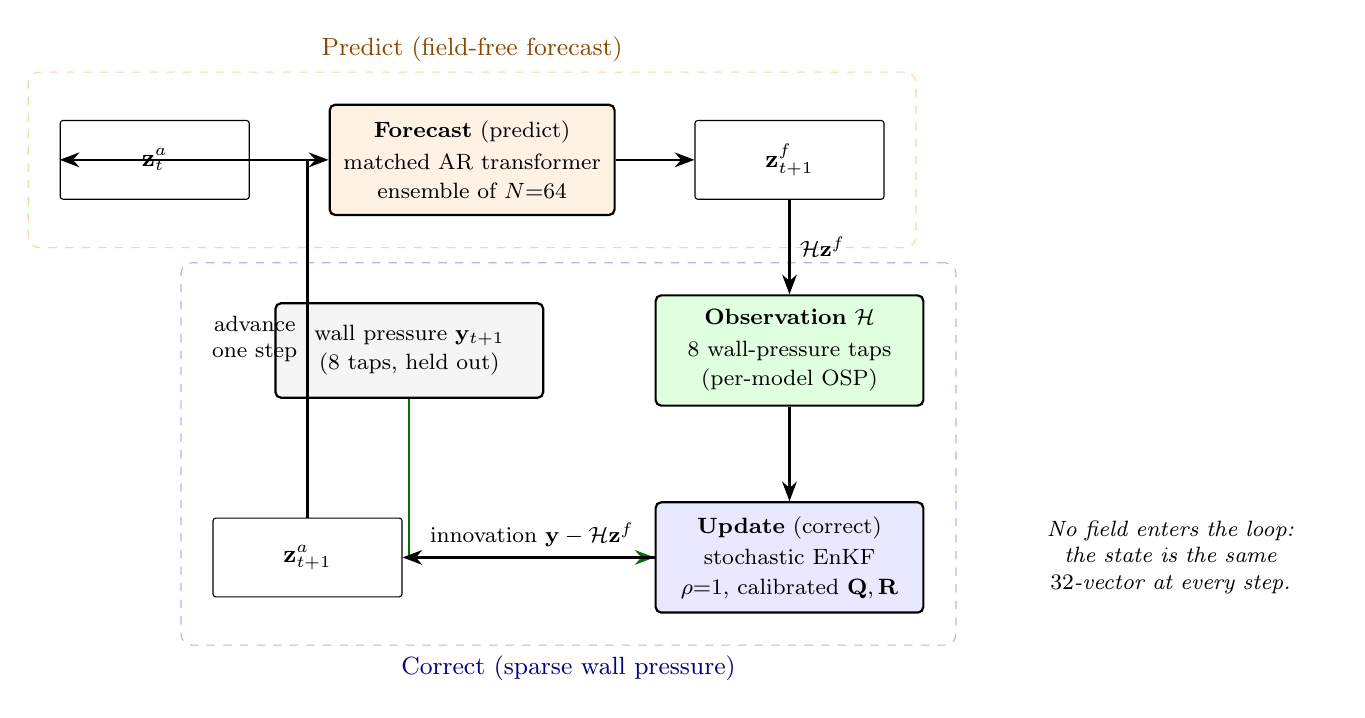
\begin{tikzpicture}[
    font=\small,
    box/.style={draw, rounded corners=2pt, align=center, inner sep=5pt, thick},
    fcst/.style={box, fill=orange!10, minimum width=36mm, minimum height=14mm,
                 font=\footnotesize},
    obsop/.style={box, fill=green!12, minimum width=34mm, minimum height=14mm,
                  font=\footnotesize},
    upd/.style={box, fill=blue!9, minimum width=34mm, minimum height=14mm,
                font=\footnotesize},
    sensor/.style={box, fill=gray!8, minimum width=34mm, minimum height=12mm,
                   font=\footnotesize},
    state/.style={draw, rectangle, rounded corners=1pt, fill=white,
                  minimum height=10mm, minimum width=24mm, inner sep=3pt},
    arr/.style={-{Stealth[length=2.5mm]}, thick},
    obsarr/.style={-{Stealth[length=2.5mm]}, thick, green!45!black}
  ]

  % ---- top row: predict ----
  \node[state] (za) {$\mathbf{z}^{a}_{t}$};
  \node[fcst, right=10mm of za] (pred)
    {\textbf{Forecast} (predict) \\[2pt]
     matched AR transformer \\[1pt]
     ensemble of $N{=}64$};
  \node[state, right=10mm of pred] (zf) {$\mathbf{z}^{f}_{t+1}$};

  \draw[arr] (za) -- (pred);
  \draw[arr] (pred) -- (zf);

  % ---- observation operator (predicted pressure) ----
  \node[obsop, below=12mm of zf] (H)
    {\textbf{Observation} $\mathcal{H}$ \\[2pt]
     $8$ wall-pressure taps \\[1pt]
     (per-model OSP)};
  \draw[arr] (zf) -- (H) node[midway, right, font=\footnotesize] {$\mathcal{H}\mathbf{z}^{f}$};

  % ---- measured wall pressure from DNS ----
  \node[sensor, left=14mm of H] (y)
    {wall pressure $\mathbf{y}_{t+1}$ \\[1pt]
     ($8$ taps, held out)};

  % ---- update (correct) ----
  \node[upd, below=12mm of H] (K)
    {\textbf{Update} (correct) \\[2pt]
     stochastic EnKF \\[1pt]
     $\rho{=}1$, calibrated $\mathbf{Q},\mathbf{R}$};
  \draw[arr] (H) -- (K);
  \draw[obsarr] (y) |- (K) node[near end, above, font=\footnotesize, black]
    {innovation $\mathbf{y}-\mathcal{H}\mathbf{z}^{f}$};

  % ---- corrected state, loop back ----
  \node[state, left=32mm of K] (zanext) {$\mathbf{z}^{a}_{t+1}$};
  \draw[arr] (K) -- (zanext);
  \draw[arr] (zanext) |- (za.west)
    node[near start, left, font=\footnotesize, align=center] {advance\\one step};

  % ---- framing note ----
  \node[align=center, font=\footnotesize\itshape, text width=40mm,
        right=10mm of K]
    {No field enters the loop: the state is the same $32$-vector at every step.};

  \begin{scope}[on background layer]
    \node[draw=orange!35, rounded corners=4pt, dashed, inner sep=4mm,
          fit=(za)(pred)(zf),
          label={[orange!55!black,font=\small]above:Predict (field-free forecast)}] {};
    \node[draw=blue!30, rounded corners=4pt, dashed, inner sep=4mm,
          fit=(y)(H)(K)(zanext),
          label={[blue!50!black,font=\small]below:Correct (sparse wall pressure)}] {};
  \end{scope}

\end{tikzpicture}

\end{document}
